\subsection{Menambahkan Kupon}
Halaman ini hanya dapat diakses oleh \textit{administrator} yang sebelumnya sudah \textit{login}. Halaman ini menampilkan form berisi elemen \textit{input} informasi kupon, dan setelah selesai lalu mengklik tombol Tambahkan Kupon, dan untuk kasus alternatif dapat dilihat pada Tabel \ref{uc06.01}.\\
\indent Tidak ada \textit{view logic} ataupun logika \textit{UI} khusus dalam halaman ini. Kode sumber implementasi \textit{back-end} dapat dilihat pada Kode Sumber \ref{cdbe.06-01}.
\newpage
\begin{lstlisting}[label=cdbe.06-01,style=php,caption=Implementasi Antarmuka Menambahkan Kupon]

/** File : app/Http/Controllers/CouponController
 * Menampilkan halaman tambah kupon
 * Method : GET
 */
public function create()
{
    $data['user'] = $this->userRepository->checkbox();
    return view('pages.coupon.create',$data);
}

/**
 * Store data kupon yang dimasukkan
 * fungsi ini dijalankan ketika form disubmit
 * terkait dengan CouponRepository
 */

public function store(Request $request)
{
    $data = $request->all();
    $data['limit_usages'] = $data['usages'];
    $ss = $this->couponRepository->storeCoupon($data);

    if($ss) return redirect('coupon')->with('success',true);
    else return redirect('coupon')->with('success',false);
}
/**
 * File CouponRepository
 */
public function storeCoupon($data)
{
	/* Menggunakan base model Laravel */
	/* return status store data ke dalam database */
    return Coupon::create($data);
}  
\end{lstlisting}
	  
      \begin{figure}[H]
        \centering
        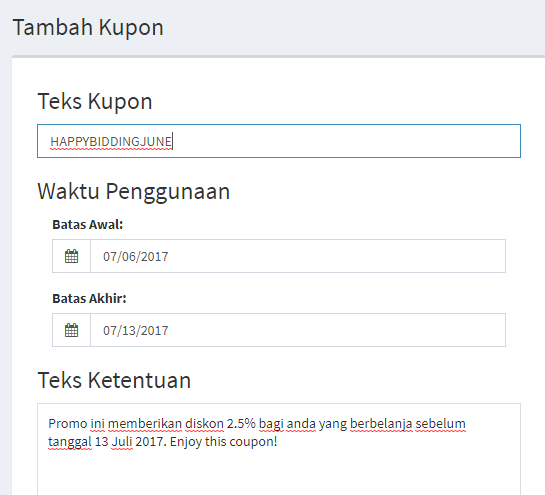
\includegraphics[width=.9\textwidth]{images/bab4/ui/06-01.png}
        \caption{Halaman Antarmuka Kasus Penggunaan Menambahkan Kupon}
        \label{ui.01-01}
      \end{figure}
      
